\documentclass[10pt]{beamer}

\usetheme[progressbar=frametitle]{metropolis}

\definecolor{ubcBlue}{RGB}{12,35,68}
\definecolor{ubcBlue1}{RGB}{0,85,183}
\definecolor{ubcBlue2}{RGB}{0,167,225}
\definecolor{ubcBlue3}{RGB}{64,180,229}
\definecolor{ubcBlue4}{RGB}{110,196,232}
\definecolor{ubcBlue5}{RGB}{151,212,223}

% \setbeamercolor{normal text}{bg=ubcBlue1}
\setbeamercolor{alerted text}{bg=ubcBlue1, fg = ubcBlue}
\setbeamercolor{example text}{fg=ubcBlue1, bg=ubcBlue1}
\setbeamercolor{title separator}{fg = ubcBlue, bg=ubcBlue}
\setbeamercolor{progress bar}{bg=ubcBlue4, fg=ubcBlue1}
\setbeamercolor{progress bar in head/foot}{bg=ubcBlue4, fg=ubcBlue1}
\setbeamercolor{progress bar in section page}{bg=ubcBlue4, fg=ubcBlue1}
\setbeamercolor{frametitle}{bg=ubcBlue}

\usepackage{amsmath}
\usepackage{amsfonts}
\usepackage{amsthm}
\usepackage{graphicx}
\usepackage{amssymb}
\usepackage{epstopdf}
\usepackage{enumerate}
\usepackage{float}
\usepackage{color}
\usepackage{soul}
\usepackage{tikz}
\usetikzlibrary{positioning,arrows,calc}

\tikzset{onslide/.code args={<#1>#2}{%
  \only<#1>{\pgfkeysalso{#2}} % \pgfkeysalso doesn't change the path
}}
\tikzset{alt/.code args={<#1>#2#3}{%
  \alt<#1>{\pgfkeysalso{#2}}{\pgfkeysalso{#3}} % \pgfkeysalso doesn't change the path
}}
\tikzset{temporal/.code args={<#1>#2#3#4}{%
  \temporal<#1>{\pgfkeysalso{#2}}{\pgfkeysalso{#3}}{\pgfkeysalso{#4}} % \pgfkeysalso doesn't change the path
}}

\DeclareMathOperator{\ord}{ord}

\usepackage{appendixnumberbeamer}

\usepackage{booktabs}
\usepackage[scale=2]{ccicons}

\usepackage{pgfplots}
\usepgfplotslibrary{dateplot}

\usepackage{xspace}
\newcommand{\themename}{\textbf{\textsc{metropolis}}\xspace}


\makeatletter
\newsavebox{\mybox}
\setbeamertemplate{frametitle}{%
  \nointerlineskip%
  \savebox{\mybox}{%
      \begin{beamercolorbox}[%
          wd=\paperwidth,%
          sep=0pt,%
          leftskip=\metropolis@frametitle@padding,%
          rightskip=\metropolis@frametitle@padding,%
        ]{frametitle}%
      \metropolis@frametitlestrut@start\insertframetitle\metropolis@frametitlestrut@end%
      \end{beamercolorbox}%
    }
  \begin{beamercolorbox}[%
      wd=\paperwidth,%
      sep=0pt,%
      leftskip=\metropolis@frametitle@padding,%
      rightskip=\metropolis@frametitle@padding,%
    ]{frametitle}%
  \metropolis@frametitlestrut@start\insertframetitle\metropolis@frametitlestrut@end%
  \hfill%
  \raisebox{-\metropolis@frametitle@padding}{
\includegraphics[height=\dimexpr\ht\mybox+\metropolis@frametitle@padding\relax]{2_2016_UBCNarrow_Signature_ReverseCMYK}}%
    \hspace*{-\metropolis@frametitle@padding}
  \end{beamercolorbox}%
}
\makeatother

%---------------------------------------------------------------------------------------------------------------------------------------------%%---------------------------------------------------------------------------------------------------------------------------------------------%

\begin{document}

%---------------------------------------------------------------------------------------------------------------------------------------------%%---------------------------------------------------------------------------------------------------------------------------------------------%

\title{Computing elliptic curves over $\mathbb{Q}$ via Thue-Mahler equations, and related problems}
\subtitle{}
% \date{\today}
\date{}
\author{Adela Gherga}
\institute{The University of British Columbia}
% \titlegraphic{\hfill\includegraphics[height=1.5cm]{logo.pdf}}

\maketitle

%---------------------------------------------------------------------------------------------------------------------------------------------%%---------------------------------------------------------------------------------------------------------------------------------------------%

\section{Thue-Mahler equations}

%---------------------------------------------------------------------------------------------------------------------------------------------%

\begin{frame}[fragile]{A definition}

\begin{itemize}
\item<1-> Let $S = \{p_1, \dots, p_v\}$ be a set of prime numbers
\item<2-> A \textit{Thue-Mahler equation} is a Diophantine equations of the form
\[F(x,y) = ap_1^{z_1}\cdots p_v^{z_v}\]
where
\begin{itemize}
\item<3-> $F(x,y) = c_0x^n + c_1x^{n-1}y + \dots + c_{n-1}xy^{n-1} + c_ny^n$
\item<4-> $a$ is a fixed integer
\item<5-> $x,y,z_1, \dots, z_v$ are unknown integers
\end{itemize}
% where F is a given binary form of degree at least $3$ and $u$ is an \textit{$S$-unit} 
% that is, an integer whose prime factors all lie in S

% degree 3 not necessary, but for out purposes, we only need degree 3 
\end{itemize}

% as it turns out, there are only finitely many solutions for any given set of coefficients and any set S
\end{frame}

%---------------------------------------------------------------------------------------------------------------------------------------------%

\begin{frame}[fragile]{Our main objective}

\centering
Given $S,F$ and $a$, find all solutions $(x,y,z_1, \dots, z_v)$ satisfying $F(x,y) = ap_1^{z_1}\cdots p_v^{z_v}$

\end{frame}

%---------------------------------------------------------------------------------------------------------------------------------------------%

\begin{frame}[fragile]{An obvious question}

Why?
\pause

\begin{itemize}
\item<2-> Compute elliptic curves
\item<3-> Solve other Diophantine equations
\item<4-> At least $4$ people heard about this project and emailed me asking for solutions to very specific Thue-Mahler equations
\end{itemize}

% We'll begin by looking at the primary motivation for our research
\end{frame}

%---------------------------------------------------------------------------------------------------------------------------------------------%

\begin{frame}[fragile]{Another obvious question}

Is this even possible?
\pause
% can we in fact find all of the solutions of a TM equation? How do we know that there are at most finitely many such solutions?
% it's a seemingly innocuous equation, but what do we know?

\begin{itemize}
\item <2-> \textbf{Mahler (1933)}: A Thue-Mahler equation has at most finitely many solutions
% in 1933, Mahler published a paper investigating Thue-Mahler equations. In this work, he generalized a classical result of Thue to prove that there are only finitely many solutions
\begin{itemize}
\item<3-> This argument is ineffective
\end{itemize}
% meaning that it provides no means to find the solutions to a TM equation
\item<4-> \textbf{Sprind\u zuk, Vinogradov, Coates (1968/1969)}:  An effective method exists to bound the number of solutions
% In 1968, a method was introduced by Baker to bound the number of solutions of a Thue equation. Generalizing Baker's ground-breaking result, Sprind\u zuk and Vinogradov \cite{SpVi} and Coates \cite{Coa} proved that the solutions could, at least in principal, be effectively determined
\item<5-> \textbf{Tzanakis, de Weger (1989)}: A practical method for solving the general Thue-Mahler equation
% The first practical method for solving the general Thue-Mahler equation over $\mathbb{Z}$ is attributed to Tzanakis and de Weger 
\item<6-> \textbf{Hambrook (2011)}: Implementation of a Thue-Mahler solver
\end{itemize}
\end{frame}

%%---------------------------------------------------------------------------------------------------------------------------------------------%
%
%\begin{frame}[fragile]{Our main result}
%
%Improved runtime!
%\pause
%
%\[F(x,y) = x^3 + 23x^2y + 17xy^2 + 2y^3 = 2^{z_1}\cdot3^{z_2}\cdot5^{z_3}\cdot7^{z_4}\cdot41^{z_5}\]
%\begin{itemize}
%
%\item <3-> \textbf{Tzanakis, de Weger: } 100 hours
%\item <3-> \textbf{Hambrook: } 687 seconds
%\item <4-> \textbf{Our new time: } 161 seconds*
%
%\end{itemize}
%\end{frame}

%---------------------------------------------------------------------------------------------------------------------------------------------%

\begin{frame}[fragile]{Going back}

Why?

\begin{itemize}
\item<1-2> Compute elliptic curves
\item<1> Solve other Diophantine equations
\item<1> At least $4$ people heard about this project and emailed me asking for solutions to very specific Thue-Mahler equations
\end{itemize}

% We'll begin by looking at the primary motivation for our research
\end{frame}

%---------------------------------------------------------------------------------------------------------------------------------------------%
%---------------------------------------------------------------------------------------------------------------------------------------------%

\section{Elliptic Curves}

%---------------------------------------------------------------------------------------------------------------------------------------------%

\begin{frame}[fragile]{Some background}

\begin{itemize}
\item<1-> An \textit{elliptic curve} is a nonsingular curve defined by
\[E: y^2 = x^3 + ax + b\]
\item<2-> A curve is nonsingular $\iff \Delta_E = 4a^3 + 27b^2 \neq 0$. 
%\item<3-> Together with the point ``at infinity'', the set of points on $E$ form a group
%\[E = \{ (x,y) \ : y^2 = x^3 + ax + b\} \cup \{\infty\}.\]
\end{itemize}

% if we consider only those points of E for which x,y in Q we obtain a subgroup of E
% and in fact, it is this subgroup that we are interested in
%  what do these subgroups look like?
\end{frame}

%---------------------------------------------------------------------------------------------------------------------------------------------%

\begin{frame}[fragile]{Visualizing subgroups of $E$}

\pause
\begin{center}
\pgfplotsset{ticks=none}
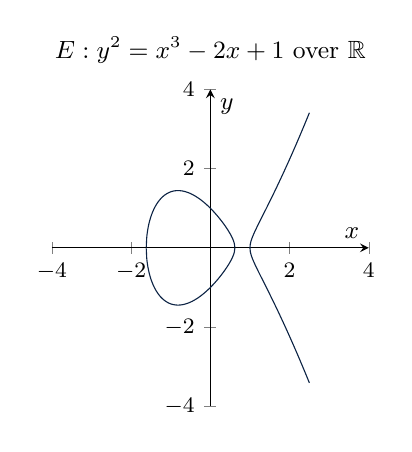
\begin{tikzpicture}[onslide=<1->]
\begin{axis}[
        xmin=-4,
        xmax=4,
        ymin=-4,
        ymax=4,
        xlabel={$x$},
        ylabel={$y$},
        axis lines=middle,
        small,
       	xtick={},      
        samples=201,
        smooth,
        font=\small,
        title={$E:y^2 = x^3 -2x + 1$ over $\mathbb{R}$},
        clip=false,
        % use same unit vectors on the axis
        axis equal image=true,
    ]
\addplot[ubcBlue, domain=1:2.5] {sqrt(x^3-2*x+1)}; 
\addplot[ubcBlue, domain=-1.618:0.618] {sqrt(x^3-2*x+1)};
\addplot[ubcBlue, domain=1:2.5] {-sqrt(x^3-2*x+1)};
\addplot[ubcBlue, domain=-1.618:0.618] {-sqrt(x^3-2*x+1)};
\end{axis}
\end{tikzpicture}\quad
\pause
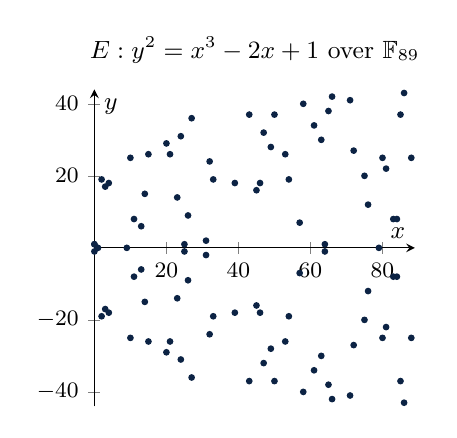
\begin{tikzpicture}[onslide=<2->]
\begin{axis}[
        xmin=0,
        xmax=89,
        ymin=-44,
        ymax=44,
        xlabel={$x$},
        ylabel={$y$},
        axis lines=middle,
        small,
       	xtick={},      
        samples=201,
        smooth,
        font=\small,
        title={$E:y^2 = x^3 -2x + 1$ over $\mathbb{F}_{89}$},
        clip=false,
        % use same unit vectors on the axis
        axis equal image=true,
    ]
    \foreach \point in {
        (0, 1), (0, 1), (0, -1), (1, 0), (2, 19), (2, -19), (3, 17), (3, -17), (4, 18), (4, -18), (9, 0),
        (10, 25), (10, -25), (11, 8), (11, -8), (13, 6), (13, -6), (14, 15), (14, -15), (15, 26), (15, -26),
        (20, 29), (20, -29), (21, 26), (21, -26), (23, 14), (23, -14), (24, 31), (24, -31), (25, 1), (25, -1), (26, 9), (26, -9), (27, 36), (27, -36),
        (31, 2), (31, -2), (32, 24), (32, -24), (33, 19), (33, -19), (39, 18), (39, -18),
        (43, 37), (43, -37), (45, 16), (45, -16), (46, 18), (46, -18), (47, 32), (47, -32), (49, 28), (49, -28),
        (50, 37), (50, -37), (53, 26), (53, -26), (54, 19), (54, -19), (57, 7), (57, -7), (58, 40), (58, -40),
        (61, 34), (61, -34), (63, 30), (63, -30), (64, 1), (64, -1), (65, 38), (65, -38), (66, 42), (66, -42),
        (71, 41), (71, -41), (72, 27), (72, -27), (75, 20), (75, -20), (76, 12), (76, -12), (79, 0),
        (80, 25), (80, -25), (81, 22), (81, -22), (83, 8), (83, -8), (84, 8), (84, -8), (85, 37), (85, -37), (86, 43), (86, -43), (88, 25), (88, -25)
      }
      \addplot[color=ubcBlue, mark=*, mark options={scale=0.5}] coordinates {\point};
      \end{axis}
\end{tikzpicture}
\end{center}

% elliptic curves over R, C, F_p, can't picture over Q (any more than we can picture Q inside R)
% over Q this is a finitely generated abelian group
% singular curves (+ conductor) discriminant 19

\end{frame}

%---------------------------------------------------------------------------------------------------------------------------------------------%

% not sure that I need this slide
\begin{frame}
\frametitle{Good and bad reduction}

\begin{itemize}
\item Reducing the coefficients of $E$ modulo $p$ yields a cubic $\tilde{E}$
\item<2-> If $\Delta_{\tilde{E}} \neq 0$ then we say that $E$ has \textit{good reduction} at $p$
% If $\tilde{E}$ is nonsingular, then it is an elliptic curve over $\mathbf{F}_p$
\item<3-> If $\Delta_{\tilde{E}} = 0$ then we say that $E$ has \textit{bad reduction} at $p$
% Otherwise we say that $E$ has \textit{bad reduction} at $p$
\end{itemize}

\begin{itemize}
\item<4->$\Delta_E = p_1^{a_1}\cdots p_n^{a_n} \implies N = p_1^{b_1}\cdots p_n^{b_n}$
\end{itemize}

\end{frame}

%---------------------------------------------------------------------------------------------------------------------------------------------%
%---------------------------------------------------------------------------------------------------------------------------------------------%

\section{Computing Elliptic Curves}

%---------------------------------------------------------------------------------------------------------------------------------------------%

\begin{frame}[fragile]{Some history}

\begin{itemize}
\item<1-> \textbf{Shafarevich (1963)}: There are at most finitely many elliptic curves having good reduction outside $S = \{p_1, \dots, p_v\}$
\item<2-> \textbf{Taniyama, Weil (1950s, 1960's)}: A conjecture about elliptic curves of conductor $N$

% in the 1950�s and 1960�s, Taniyama and Weil asked whether all elliptic curves over Q of a given conductor N are related to modular functions.

% While this conjecture is now known as the Modularity Theorem, until its proof in 2001, attempts to verify it sparked a large effort to tabulate all elliptic curves over Q of given conductor N.

\begin{itemize}
\item <3->$S = \{2\}$: Ogg ($1966$) 
%determined all elliptic curves defined over $\mathbb{Q}$ with conductor of the form $2^a$. 

\item <3->$S = \{2,3\}$: Coghlan ($1967$)
%in his dissertation \cite{Coghlan}, studied the curves of conductor $2^a3^b$ independently of Ogg, 

\item <3->$S = \{p\}$ for certain small primes $p$: Setzer ($1975$)
%while Setzer \cite{Setzer} computed all $\mathbb{Q}$-isomorphism classes of elliptic curves of conductor $p$ for certain small primes $p$. 

\item <3->$S = \{11\}$: Agrawal, Coates, Hunt, and van der Poorten ($1980$)
%determined all elliptic curves of conductor $11$ defined over $\mathbb{Q}$ to verify the (then) conjecture of Taniyama-Weil for $N= 11$.

\end{itemize}


\end{itemize}

\end{frame}

% Let $K$ be a number field and let $S$ be a finite set of places of $K$ containing the infinite places. 

% In $1963$ Shafarevich proved that there are at most finitely many $K$-isomorphism classes of elliptic curves defined over $K$ having good reduction outside $S$.


% All of these early attempts have much in common in that they often reduce the problem to one of solving a number of certain integral binary forms called Thue-Mahler equations. 



%---------------------------------------------------------------------------------------------------------------------------------------------%
%
%\begin{frame}[fragile]{Our motivation}
%
%\centering
%Given $S$, find all such curves explicitly!
%
%% This is the question that ultimately leads us back to our primary objective of solving Thue-Mahler equations
%% Before we go into the details of how this is done and what the connection is to Thue-Mahler equations, let's ask the obvious question again: why?
%% Before we go into the details of how this is to be done, look at some historical data
%
%\end{frame}

%---------------------------------------------------------------------------------------------------------------------------------------------%
%
%\begin{frame}[fragile]{Some history}
%
%\begin{itemize}
%\item <1-> Taniyama, Weil (1950s, 1960's): Are all $E/\mathbb{Q}$ of a given conductor $N$ related to modular functions?
%
%% in the 1950�s and 1960�s, Taniyama and Weil asked whether all elliptic curves over Q of a given conductor N are related to modular functions.
%
%% While this conjecture is now known as the Modularity Theorem, until its proof in 2001, attempts to verify it sparked a large effort to tabulate all elliptic curves over Q of given conductor N.
%
%\begin{itemize}
%\item <2->$S = \{2\}$: Ogg ($1966$) 
%%determined all elliptic curves defined over $\mathbb{Q}$ with conductor of the form $2^a$. 
%
%\item <2->$S = \{2,3\}$: Coghlan ($1967$)
%%in his dissertation \cite{Coghlan}, studied the curves of conductor $2^a3^b$ independently of Ogg, 
%
%\item <2->$S = \{p\}$ for certain small primes $p$: Setzer ($1975$)
%%while Setzer \cite{Setzer} computed all $\mathbb{Q}$-isomorphism classes of elliptic curves of conductor $p$ for certain small primes $p$. 
%
%\item <2->$S = \{11\}$: Agrawal, Coates, Hunt, and van der Poorten ($1980$)
%%determined all elliptic curves of conductor $11$ defined over $\mathbb{Q}$ to verify the (then) conjecture of Taniyama-Weil for $N= 11$.
%
%\end{itemize}
%\end{itemize}
%
%% All of these early attempts have much in common in that they often reduce the problem to one of solving a number of certain integral binary forms called Thue-Mahler equations. 
%
%\end{frame}

%---------------------------------------------------------------------------------------------------------------------------------------------%

\begin{frame}[fragile]{The modern approach}

% There are very few, if any, subsequent attempts in the literature to find elliptic curves of given conductor via Thue-Mahler equations. 

% Instead, many of the approaches involve a completely different method to the problem, using modular forms. 

% This method relies upon the Modularity Theorem, which was still a conjecture (under various guises) when these ideas were first implemented. Much of the success of this approach can be attributed to Cremona and his collaborators, who have devoted decades of work to it. In fact, using this method, all elliptic curves over $\mathbb{Q}$ of conductor $N$ have been determined for values of $N$ as follows

% Cremona between 1988 - 2017

\begin{itemize}
\item<1-> Subsequent methods rely on the Modularity Theorem
\item<2-> All elliptic curves of conductor $N$ have been determined for

\begin{itemize} \itemsep0em
\item<3-> Antwerp IV ($1972$): $N \leq 200$
\item<3-> Tingley ($1975$): $N \leq 320$
\item<3-> Cremona ($2019$): $N \leq 500000$
\end{itemize}
\end{itemize}

% In our present work, we will instead return to techniques based upon solving Thue-Mahler equations. 

\end{frame}

%---------------------------------------------------------------------------------------------------------------------------------------------%

\begin{frame}[fragile]{The Thue-Mahler approach}

\begin{itemize}
% More precisely, fix K and S
%\item<1-> Let $S = \{p_1, \dots, p_v\}$ be a set of prime numbers

% In the 1970's, Coates provided the first effective proof of Shafaravich�s Theorem, for the the special case K = Q and S = {2, 3}

% We note that early attempts to compute ECs with good reduction outside S have much in common with the approach used by Coates 

% in that they often reduce the problem to one of solving a number of Thue-Mahler equations.

\item<1-> Reduce problem to solving a number of Thue-Mahler equations 
\[F(x,y) = c_0x^3 + c_1x^2y + c_2xy^2 + c_3y^3 = ap_1^{z_1}\cdots p_v^{z_v}\]

% where F is a given binary form of degree at least $3$ and $u$ is an \textit{$S$-unit} 
% that is, an integer whose prime factors all lie in S

% Find $\varepsilon_{\mathbb{Q}, S}$ explicitly via Thue-Mahler equations

%\begin{itemize}
%\item<3-> Implementation of a TM equation solver based on Tzanakis, de Weger
%\end{itemize}

\item<2> Goal: compute all curves having conductor $N \leq 10^6$
\item<3-> Ideal Goal: $N \leq 10^8$
\end{itemize}

% In our research, we have implemented a computer program which generates all elliptic curves over $K$ having good reduction outside $S$ and bounded conductor. 
% This algorithm is based on the work of de Weger, Tzanakis, following the work of BeRe


\end{frame}

%---------------------------------------------------------------------------------------------------------------------------------------------%
%
%\begin{frame}[fragile]{An overview of the theorem} 
%
%% a theorem by Bennett and Rechnitzer (who has asked to not be mentioned) illustrates the connection between elliptic curves over Q and cubic forms, 
%% and leads us to the algorithm for determining all elliptic curves over Q of conductor N
%
%% this theorem is technical;  
%
%\begin{itemize}
%%\item<1-> Let $K = \mathbb{Q}$ and $S = \{p_1, \dots, p_v\}$ be a set of rational primes. \\
%% suppose we want to find an EC with conductor N
%
%\item<1-> Compute $E/\mathbb{Q}$ with good reduction outside $S = \{p_1, \dots, p_v\}$ 
%\begin{itemize}
%\item<2-> $\Leftrightarrow$ find $E/\mathbb{Q}$ with conductor $N = p_1^{a_1}\cdots p_v^{a_v}$, $a_i \in \mathbb{N}$\\ 
%\end{itemize}
%%\Leftrightarrow$ find $E/\mathbb{Q}$ with conductor $N = p_1^{a_1}\cdots p_v^{a_v}$, $a_i \in \mathbb{N}$\\ 
%% there exists an integral binary cubic form F with discriminant $N_0$ "dividing" $N$ and relatively prime integers u,v with 
%
%\item<2-> For $N_0 \mid 12 N$, there exists 
%\[F(u,v) = c_0u^3 + c_1u^2v + c_2uv^2 + c_3v^3 = 2^{\alpha_1}3^{\beta_1}\prod_{p|N_0}p^{\kappa_p}\]
%with discriminant $N_0$
%
%\item <3-> Then $E \cong_{\mathbb{Q}} E_{\mathcal{D}}$, where $E_{\mathcal{D}}$ is determined by the form $F$ and $(u,v)$
%\end{itemize}
%\end{frame}

% prime database has 400bilion/trillion? a lot

% algorithmically can write down forms in linear time

%We note that there might exist such a form $F$ and corresponding $E_{\mathcal{D}}$, but it may be the case that conductor $N_{E_{\mathcal{D}}} \neq N$. This can occur if certain local conditions at $2$ are not satisfied. 

% Additionally, if the curve $E$ has at least one rational $2$-torsion point, the cubic forms arising from this theorem will necessarily be reducible. 

% easier if has 2 torsion, or if prime case (thue)


%---------------------------------------------------------------------------------------------------------------------------------------------%

\begin{frame}[fragile]{The theorem}

% More precisely

\begin{theorem}[Bennett, G., Rechnitzer] \label{BeRe}
Let $E/\mathbb{Q}$ be an elliptic curve of conductor $N = 2^{\alpha}3^{\beta}N_0$ where $N_0$ is coprime to $6$.
% and suppose $j_E \neq 0$

Then there exists an integral binary cubic form $F$ of discriminant
\[D_F = \text{sign}(\Delta_E)2^{\alpha_0}3^{\beta_0}N_1,\] 
and relatively prime integers $u$ and $v$ with 
\[F(u,v) = c_0u^3 + c_1u^2v + c_2uv^2 + c_3v^3 = 2^{\alpha_1}3^{\beta_1}\prod_{p|N_0}p^{\kappa_p}\]

such that $E$ is isomorphic over $\mathbb{Q}$ to $E_{\mathcal{D}}$, where
\[E_{\mathcal{D}} : 3^{[\beta_0/3]} y^2 = x^3 - 27\mathcal{D}^2 H_F(u,v)x + 27\mathcal{D}^3G_F(u,v).\]
\end{theorem}

\end{frame}
% $0 \leq \alpha \leq 8$, $0 \leq \beta \leq 5$. S
% square brackets [r] mean that its the greatest integer not exceeding the real number r

\begin{frame}
\begin{theorem}[Bennett, G., Rechnitzer]
%\vspace*{-\baselineskip}\setlength\belowdisplayshortskip{0pt}
Here, $N_1\mid N_0$,
\[ (\alpha_0, \alpha_1) = 
\begin{cases}  
	(2,0) \text{ or } (2,3)  & \text{ if } \alpha = 0 \\
	(3,\geq 3) \text{ or } (2,\geq 4)  & \text{ if } \alpha = 1 \\
	(2,1), (4,0) \text{ or } (4,1)  & \text{ if } \alpha = 2 \\
	(2,1), (2,2), (3,2), (4,0) \text{ or } (4,1)  & \text{ if } \alpha = 3 \\
	(2,\geq 0), (3,\geq 2), (4,0) \text{ or } (4,1)  & \text{ if } \alpha = 4 \\
	(2,0) \text{ or } (3,1)  & \text{ if } \alpha = 5 \\
	(2,\geq 0), (3,\geq 1), (4,0) \text{ or } (4,1)  & \text{ if } \alpha = 6 \\
	(3,0) \text{ or } (4,0)  & \text{ if } \alpha = 7 \\
	(3,1) & \text{ if } \alpha = 8,
\end{cases} \]
\end{theorem}
\end{frame}

\begin{frame}
\begin{theorem}[Bennett, G., Rechnitzer]
\[ (\beta_0, \beta_1) = 
\begin{cases}  
	(0,0) & \text{ if } \beta = 0 \\
	(0,\geq 1) \text{ or } (1,\geq 0) & \text{ if } \beta = 1 \\
	(3,0), (0,\geq 0), \text{ or } (1,\geq 0)  & \text{ if } \beta = 2 \\
	(\beta,0) \text{ or } (\beta,1)  & \text{ if } \beta \geq 3,
\end{cases} \]
% non-negative integers, where $alpha \in [0,8]$ and $\beta \in [0,5]
\[\mathcal{D} = \prod_{p|\gcd(c_4(E),c_6(E))} p^{\min\{ [\nu_p(c_4(E))/2], [\nu_p(c_6(E))/3] \}},\]
and $\kappa_p \in \mathbb{Z}_{>0}$ with $\kappa_p \in \{0,1\}$ whenever $p^2|N_{1}$.
% excluding some additional details that we know about kappas here
%\[\text{ and } \kappa_p \in \mathbb{Z}_{>0} \text{ with } \nu_p(\Delta_E) = 
%\begin{cases}
%	\nu_p(D_F) + 2\kappa_p & \text{ if } p \nmid \mathcal{D} \\
%	\nu_p(D_F) + 2\kappa_p + 6 & \text{ if } p \mid \mathcal{D},
%\end{cases}\]
%and 
%\[\kappa_p \in \{0,1\} \text{ whenever } p^2|N_{1}.\]

Further, 
\[\text{ if } \beta_0 \geq 3, \text{ then } 3|c_1 \text{ and } 3|c_2\] 
and 
\[\text{ if } \nu_p(N) = 1, \text{ for } p \geq 3, \text{ then } p \mid D_FF(u,v)\]
\end{theorem} 

\end{frame}

%---------------------------------------------------------------------------------------------------------------------------------------------%

\begin{frame}[fragile]{The algorithm}

%Using this theorem, we may compute all $E/\mathbb{Q}$ of conductor $N$ via the following algorithm:
\begin{enumerate}
\item<2-4> Compute every binary form $F$ as given in the statement of the theorem \\
%Compute $GL_2({\mathbb{Z}})$-representatives for every binary form $F$ with discriminant
%\[D_F = \pm 2^{\alpha_0}3^{\beta_0}N_1\]
%for each divisor $N_1$ of $N_0$, and each possible pair $(\alpha_0,\beta_0)$ given in the statement of the theorem  \\  
\item<3-5> Solve the corresponding Thue-Mahler equations \\
\item<4> Check ``local" conditions and output the elliptic curves that arise
\end{enumerate}  


% the first and the third of these steps are straightforward. 

% Indeed, in  Bennett and Rechnitzer describe an efficient algorithm for carrying out Step 1, 
% and Step 3 is essentially trivial. 

% The bulk of the work is concentrated in Step 2. This is the main focus of this report and in fact one of the main objective of this research. The remaining chapters of this report are devoted to carrying out this step. 

% We carried out a one-time computation of all irreducible cubic forms that can arise in Theorem 1, of abso- lute discriminant bounded by 10^10. There are ?? such forms; storing them takes ?? space.

% 120 gigs to store, big computation, took couple of days, (forms conductor up to 10^10)
% but now have the forms - one time computation
% simply storing it, past this
% been done! hence, trivial, just a matter of table look-up
% can happen that there are no forms (happens quite a lot; a positive proportion of the time)


\end{frame}

%---------------------------------------------------------------------------------------------------------------------------------------------%

\begin{frame}[fragile]{Representative forms: an example}

\begin{itemize}
\item<1-> Let $S = \{2,3,5,7,11,13\}$
\item<2-> There are 7893 corresponding forms which need to be solved
\begin{itemize}
\item<3->$F(x,y) = 19x^3 + 69x^2y + 76xy^2 + 126y^3 = 2^{z_1}\cdot 3^{z_2}\cdot 5^{z_3}\cdot 7^{z_4}\cdot 11^{z_5}\cdot 13^{z_6}$
\item<3-> $F(x,y) = 22x^3 + 22x^2y + 55xy^2 + 100y^3 = 2^{z_1}\cdot 3^{z_2}\cdot 5^{z_3}\cdot 7^{z_4}\cdot 11^{z_5}\cdot 13^{z_6}$
\item<3-> $F(x,y) = 46x^3 + 24x^2y + 85xy^2 + 7y^3 = 2^{z_1}\cdot 3^{z_2}\cdot 5^{z_3}\cdot 7^{z_4}\cdot 11^{z_5}\cdot 13^{z_6}$
\item<3-> $F(x,y) = 13x^3 + 3x^2y + 18xy^2 + 14y^3 = 2^{z_1}\cdot 3^{z_2}\cdot 5^{z_3}\cdot 7^{z_4}\cdot 11^{z_5}\cdot 13^{z_6}$
\item<3-> $F(x,y) = 17x^3 + 36x^2y + 39xy^2 + 26y^3 = 2^{z_1}\cdot 3^{z_2}\cdot 5^{z_3}\cdot 7^{z_4}\cdot 11^{z_5}\cdot 13^{z_6}$
\item<3-> $F(x,y) = 2x^3 + 18x^2y + 21xy^2 + 65y^3 = 2^{z_1}\cdot 3^{z_2}\cdot 5^{z_3}\cdot 7^{z_4}\cdot 11^{z_5}\cdot 13^{z_6}$
\item<3-> $F(x,y) = x^3 + 12x^2y + 18xy^2 + 149y^3 = 2^{z_1}\cdot 3^{z_2}\cdot 5^{z_3}\cdot 7^{z_4}\cdot 11^{z_5}\cdot 13^{z_6}$ \\
\[\vdots\]
\end{itemize}

\end{itemize}

% one-time computation
% split into irreducible, reducible

% trying to do this for every set of primes whose product is less than 10^6
% this might be worrisome, but how bad is it?

\end{frame}

%---------------------------------------------------------------------------------------------------------------------------------------------%
%---------------------------------------------------------------------------------------------------------------------------------------------%

\section{Applying the Thue-Mahler solver}

%---------------------------------------------------------------------------------------------------------------------------------------------%

\begin{frame}
\frametitle{Some timing examples}
%using tzanakis de Wegers approach

\begin{itemize}
\item<1-> A nice example
\[x^3 + 3xy^2 + 44xy^2 + 66y^3 = 3^{z_1}\cdot 11^{z_2}\cdot17^{z_3}\cdot23^{z_4}\cdot31^{z_5}\]
\only<2->{Total time: 247.580}

\item<1-> A less nice example
\[3x^3 + 3xy^2 + 44xy^2 + 66y^3 = 3^{z_1}\cdot11^{z_2}\cdot17^{z_3}\cdot23^{z_4}\cdot31^{z_5}\]
\only<2->{Total time: 2031.450} \\ % 1.6hrs \\

\end{itemize}

\end{frame}

% should convince you that this doesn't look promising, but why? what's going on?
% the prognosis doesn't look good
% can't use westgrid

%---------------------------------------------------------------------------------------------------------------------------------------------%
%---------------------------------------------------------------------------------------------------------------------------------------------%

\section{Algorithms for solving Thue-Mahler equations}

%---------------------------------------------------------------------------------------------------------------------------------------------%

\begin{frame}<1>[label=overview]
\frametitle{Overview}

\begin{figure}
\centering

\tikzstyle{block} = [rectangle, fill=ubcBlue,
    text=structure.bg, text centered, rounded corners, minimum height=1.5em, minimum width=5em ]
\tikzstyle{line} = [line width=0.5pt, -triangle 45, color=ubcBlue]
\tikzstyle{linealert} = [line width=0.5pt, -triangle 45, color=ubcBlue1]
\tikzstyle{linedim} = [line width=0.5pt, -triangle 45, color=ubcBlue!30]
\tikzstyle{alert} = [text=structure.bg, fill=ubcBlue1]
\tikzstyle{dim} = [text=structure.bg, fill=ubcBlue!30]

\begin{tikzpicture}[node distance=1.5cm, auto]
\usebeamercolor{frametitle}
    % Place nodes
    \node [block,onslide=<2>{dim},onslide=<3-4>{alert}] (S) {\small Set of Primes};
    \node []				             (F1m) [right of =S, node distance=2cm] { $\quad \vdots$};
    \node [] 				     (Filler1) [above of =F1m, node distance=0.4cm] {};
    \node [] 				     (Filler2) [below of =F1m, node distance=0.4cm] {};
    \node [block,onslide=<2-3>{dim},onslide=<4>{alert}] (F1)[above of =Filler1, node distance = 0.9cm] {\small TM Eq $\mu$};
    \node [block,onslide=<2-3>{dim},onslide=<4-6>{alert}] (Fm) [below of =Filler2,node distance = 0.9cm ] {\small TM Eq $1$};
    \node [] 				     (F12m) [right of =Fm, node distance=2cm] { $\vdots$};
    \node [] 				     (Filler3) [above of =F12m, node distance=0.4cm] {};
    \node [] 				     (Filler4) [below of =F12m, node distance=0.4cm] {};
    \node [block,onslide=<2-5>{dim},onslide=<6>{alert}] (F21)[above of =Filler3, node distance = 0.9cm] {\small Monic Eq $m$};
    \node [block,onslide=<2-5>{dim},onslide=<6-8>{alert}] (F2m) [below of =Filler4, node distance = 0.9cm] {\small Monic Eq $1$};
    \node [] 				     (ideal1m) [right of =F2m, node distance=2cm] { $\vdots$};
    \node [] 				     (Filler5) [above of =ideal1m, node distance=0.4cm] {};
    \node [] 				     (Filler6) [below of =ideal1m, node distance=0.4cm] {};
    \node [block,onslide=<2-7>{dim},onslide=<8>{alert}] (ideal1)[above of =Filler5, node distance = 0.9cm] {\small Ideal Eq $M$};
    \node [block,onslide=<2-7>{dim}, onslide=<8-10>{alert}] (idealm) [below of =Filler6, node distance = 0.9cm] {\small Ideal Eq $1$};
    \node [] 				     (S1m) [right of =idealm, node distance=2cm] { $\vdots$};
    \node [] 				     (Filler7) [above of =S1m, node distance=0.4cm] {};
    \node [] 				     (Filler8) [below of =S1m, node distance=0.4cm] {};
    \node [block,onslide=<2-9>{dim}, onslide=<10>{alert}] (S1)[above of =Filler7, node distance = 0.9cm] {\small $S$-unit Eq $\mathcal{M}$};
    \node [block,onslide=<2->{dim},onslide=<10-11>{alert}] (Sm) [below of =Filler8, node distance = 0.9cm] {\small $S$-unit Eq 1};

    \draw [line,onslide=<2-3>{linedim},onslide=<4>{linealert}] (S) -> (F1);
    \draw [line,onslide=<2-3>{linedim},onslide=<4>{linealert}] (S) -> (Fm);
    \draw [line,onslide=<2-3>{linedim},onslide=<4>{linealert}] (S) -> (F1m);
    \draw [line,onslide=<2-3>{linedim},onslide=<4>{linealert}] (S) -> (Filler1);
    \draw [line,onslide=<2-3>{linedim},onslide=<4>{linealert}] (S) -> (Filler2);
    \draw [line,onslide=<2-5>{linedim},onslide=<6>{linealert}] (Fm) -> (F21);
    \draw [line,onslide=<2-5>{linedim},onslide=<6>{linealert}] (Fm) -> (F2m);
    \draw [line,onslide=<2-5>{linedim},onslide=<6>{linealert}] (Fm) -> (F12m);
    \draw [line,onslide=<2-5>{linedim},onslide=<6>{linealert}] (Fm) -> (Filler3);
    \draw [line,onslide=<2-5>{linedim},onslide=<6>{linealert}] (Fm) -> (Filler4);
    \draw [line,onslide=<2-7>{linedim}, onslide=<8>{linealert}] (F2m) -> (ideal1);
    \draw [line,onslide=<2-7>{linedim},onslide=<8>{linealert}] (F2m) -> (idealm);
    \draw [line,onslide=<2-7>{linedim},onslide=<8>{linealert}] (F2m) -> (ideal1m);
    \draw [line,onslide=<2-7>{linedim},onslide=<8>{linealert}] (F2m) -> (Filler5);
    \draw [line,onslide=<2-7>{linedim},onslide=<8>{linealert}] (F2m) -> (Filler6);
    \draw [line,onslide=<2-9>{linedim}, onslide=<10>{linealert}] (idealm) -> (S1);
    \draw [line, onslide=<2-9>{linedim}, onslide=<10>{linealert}] (idealm) -> (Sm);
    \draw [line,onslide=<2-9>{linedim}, onslide=<10>{linealert}] (idealm) -> (S1m);
    \draw [line,onslide=<2-9>{linedim}, onslide=<10>{linealert}] (idealm) -> (Filler7);
    \draw [line,onslide=<2-9>{linedim}, onslide=<10>{linealert}] (idealm) -> (Filler8);

\end{tikzpicture}
\end{figure}
\end{frame}

%---------------------------------------------------------------------------------------------------------------------------------------------%

\againframe<2>{overview}

\againframe<3>{overview}

\againframe<4>{overview}

\againframe<5>{overview}

%---------------------------------------------------------------------------------------------------------------------------------------------%

\begin{frame}
\frametitle{First steps}

%practical method for solving a Thue-Mahler equation over Z
% \item Large upper bound for the solutions is derived via the theory of linear forms in logs 
% \item The upper bound is considerably reduced by diophantine approximation computations, based on applying the LLL algorithm to approximation lattices related to the linear forms, both in the real/complex and $p$-adic case
%\ item The solutions below the reduced bound can be found by several methods: Fincke-Pohst, a sieving process, and enumeration of the possibilities. (Main bottleneck)

\begin{itemize}
\item<1-3> Fix $a \in \mathbb{Z}$ and a set of distinct rational primes $S = \{p_1, \dots, p_v\}$
% fix a non-zero integer a and a set of distinct rational primes  
\item<1-> Reduce problem to solving a number of \textit{Thue-Mahler equations},
\only<1-2> {
\[F(x,y) = c_0x^3 + c_1x^2y + c_2xy^2 + c_3y^3 = a p_1^{z_1} \cdots p_v^{z_v}\]}
% for unknown integers $x,y,z_1, \dots, z_v$ with $z_i \geq 0$
% irreducible binary form over Z
\only<3> {
\[F(x,y) = x^3 + c_1x^2y + c_2xy^2 + c_3y^3  = a p_1^{z_1} \cdots p_v^{z_v}\]}
%for unknown integers $x,y,z_1, \dots, z_v$ with $z_i \geq 0$
\item<2-3> Without loss of generality, we may assume
\only<2> 
{\[(x,y) = (y,c_0) = 1 \quad \text{ and } \quad (a, p_1, \dots, p_v) = 1\]}
\only<3>
{\[(x,y) = 1 \quad \text{ and } \quad (a, p_1, \dots, p_v) = 1\]}

\end{itemize}

% this is fine in our case, f_0 = 1
%\end{itemize}
% explanation of coefficient business here

% based on work by Tzanakis, de Weger
% GL2Z ISSUES MENTIONED HERE
% timing example

\end{frame}

%---------------------------------------------------------------------------------------------------------------------------------------------%

\againframe<5>{overview}

\againframe<6>{overview}

\againframe<7>{overview}

%---------------------------------------------------------------------------------------------------------------------------------------------%

\begin{frame}[fragile]{The setup}
\frametitle{The setup}

\begin{itemize}
% practical method for solving a Thue-Mahler equation over Z
\item<1-> Generate a number field $K$
%Put $g(t) = F(t,1) = t^3 + c_1 t^{2} + c_2 t + c_3$ 
%and note that $g(t)$ is irreducible in $\mathbb{Z}[t]$. 
%\item<2-> Let $K = \mathbb{Q}(\theta)$ with $g(\theta) = 0$
\item<2-> Solving $F(x,y) = a p_1^{z_1} \cdots p_v^{z_v}$ is equivalent to solving  a set of \textit{ideal equations}
\[(x-y\theta)\mathcal{O}_K = \mathfrak{a}\mathfrak{p}_{1}^{u_{1}}\cdots \mathfrak{p}_{\nu}^{u_{\nu}}\]

where
\begin{itemize}
\item<3->$\mathfrak{a}, \mathfrak{p}_{i} $ are determined by $a, p_i$
\item<4->$x,y,u_i$ are unknown non-negative integers to be solved for
\end{itemize}
\end{itemize}

 %can reduce the number of variables appearing here: ie. anything with e_if_i > 1 has an upper bound
\end{frame}

%---------------------------------------------------------------------------------------------------------------------------------------------%
%
%\begin{frame}
%\frametitle{The prime ideal removing lemma}
%
%\begin{itemize}
%\item Applying the PIRL, we are left with a set of \textit{ideal equations}
%\[(x-y\theta)\mathcal{O}_K = \mathfrak{a}\mathfrak{p}_{1}^{u_{1}}\cdots \mathfrak{p}_{\nu}^{u_{\nu}}\]
%
%% in integer variables $X,u_1, \dots, u_v$ with $u_i \geq 0$ for $i = 1, \dots, v$. Here
%% basterdizing notation hard here
%\begin{itemize}
%\item<2-> $\mathfrak{a}, \mathfrak{p}_i$ are ideals determined by $a, p_i$
%\item<3-> $x,y,u_i $ are unknown non-negative integers to be solved for
%\end{itemize}
%\end{itemize}
%\end{frame}

% There are further refinements here so that we can reduce some of these equations further
%ADD MORE DETAIL HERE
% the details of what this means doesn't necessarily matters; what does is that we've now forked again

%---------------------------------------------------------------------------------------------------------------------------------------------%

\againframe<7>{overview}

\againframe<8>{overview}

%---------------------------------------------------------------------------------------------------------------------------------------------%

\begin{frame}
\frametitle{Example: the number of ideal equations}

\begin{itemize}
\item<1-> A nice example
\[x^3 + 20xy^2 + 24xy^2 + 15y^3 = 2^{z_1}\cdot 3^{z_2}\cdot 17^{z_3}\cdot 37^{z_4}\cdot53^{z_5}\]
\item<2>{Number of Ideal Equations: 32} \\ % 1.6hrs

\item<1-> A less nice example
\[7x^3 + xy^2 + 29xy^2 - 25y^3 = 2^{z_1}\cdot 3^{z_2}\cdot 17^{z_3}\]
\item<2>{Number of Ideal Equations: 26,136} \\ 

\end{itemize}

\end{frame}

%---------------------------------------------------------------------------------------------------------------------------------------------%

\againframe<8>{overview}

\againframe<9>{overview}

%---------------------------------------------------------------------------------------------------------------------------------------------%

\begin{frame}[fragile]{Principalization tests}

\begin{itemize}
\item<1-> Applying a number of principalization tests, we are left with a set of \textit{$S$-unit equations}
\[x-y\theta = \alpha \varepsilon_1^{a_1}\cdots \varepsilon_r^{a_r}\gamma_1^{n_1} \cdots \gamma_{\nu}^{n_{\nu}}\]
\begin{itemize}
\item<2->$ \alpha, \varepsilon_i, \gamma_i$ are computed directly from the ideal equation
\item<3-> $x,y,a_i, n_i$ are unknown
\end{itemize}
\end{itemize}

\end{frame}

%---------------------------------------------------------------------------------------------------------------------------------------------%

\againframe<9>{overview}

\againframe<10>{overview}

%---------------------------------------------------------------------------------------------------------------------------------------------%
\begin{frame}[fragile]{Example: the number of $S$-unit equations}

\begin{itemize}
\item A nice example
\[7x^3 + 12xy^2 +14y^3 = 7^{z_1}\cdot 11^{z_2}\cdot 37^{z_3}\]
\only<1->{\textbf{Number of ideal equations}: 16} 

\only<1->{\textbf{Number of principalization tests}: 11,664} 

\only<1->{\textbf{Number of $S$-unit equations}: 1296} % 1second 

\only<1->{\textbf{Total time}: 21.5 seconds} 

\end{itemize}
\end{frame}
% worst case scenario of h^v cases, and h_i = 9 for all 3 prime ideals

%---------------------------------------------------------------------------------------------------------------------------------------------%

\begin{frame}[fragile]{Example: the number of $S$-unit equations}

\begin{itemize}
\item A less nice example
\only
\[2x^3 + 20x^2y - 14xy^2 + 37y^3 = 2^{z_1}\cdot 3^{z_2}\cdot 5^{z_3}\cdot 11^{z_4} \cdot 13^{z_5} \cdot 17^{z_6}\]
\only<1->{\textbf{Number of ideal equations}: 448} 

\only<1->{\textbf{Number of principalization tests}: 7,560,000} 

\only<1->{\textbf{Number of $S$-unit equations}: 139,264} % 1second 

\only<1->{\textbf{Total time}: 4 hours}

\end{itemize}
\end{frame}

%---------------------------------------------------------------------------------------------------------------------------------------------%

\begin{frame}[fragile]{Example: the number of $S$-unit equations}

\begin{itemize}
\item A really, really bad example
\[14x^3 + 20x^2y + 24xy^2 + 15y^3 = 2^{z_1}\cdot 3^{z_2}\cdot 17^{z_3}\cdot 37^{z_4} \cdot 53^{z_5}\]

\only<1->{\textbf{Number of ideal equations}: 64} 

\only<1->{\textbf{Number of principalization tests}: 113,848,416} 

\only<1->{\textbf{Number of $S$-unit equations}: ????} % 1second 

\only<1->{\textbf{Total time}: ????} 

\end{itemize}
\end{frame}

%---------------------------------------------------------------------------------------------------------------------------------------------%

\againframe<10>{overview}

\againframe<11>{overview}

%---------------------------------------------------------------------------------------------------------------------------------------------%

\begin{frame}
\frametitle{For each $S$-unit equation...}

\begin{itemize}
\item Generate a very large upper bound on the solutions
\item Reduce this bound 
\begin{itemize}
\item Compute all short vectors in a lattice
\end{itemize}
\item Search below this reduced bound 
\end{itemize}
% maybe mention FP, short vectors processes 
\end{frame}

%---------------------------------------------------------------------------------------------------------------------------------------------%
%---------------------------------------------------------------------------------------------------------------------------------------------%

\section{Refined algorithms for solving Thue-Mahler equations}

%---------------------------------------------------------------------------------------------------------------------------------------------%

\againframe<1>{overview}

\againframe<2>{overview}

\againframe<3>{overview}

\againframe<4>{overview}

\againframe<5>{overview}

\againframe<6>{overview}

\againframe<7>{overview}

%---------------------------------------------------------------------------------------------------------------------------------------------%

\begin{frame}[fragile]{Our refinements}

\begin{itemize}
\item<1-> Fewer ideal equations
\item<2-> Fewer $S$-unit equations
\begin{itemize}
\item<3-> Reduced test run-time
\item<4-> Yields only 1 $S$-unit equation for each ideal equation
\end{itemize}
\item<5-> Faster bound reduction for each $S$-unit equation
\end{itemize}

\end{frame}

%---------------------------------------------------------------------------------------------------------------------------------------------%

\againframe<7>{overview}

\againframe<8>{overview}

\againframe<9>{overview}

%---------------------------------------------------------------------------------------------------------------------------------------------%

\begin{frame}<1>[label=overview2]
\frametitle{Overview}

\begin{figure}
\centering

\tikzstyle{block} = [rectangle, fill=ubcBlue,
    text=structure.bg, text centered, rounded corners, minimum height=1.5em, minimum width=5em ]
\tikzstyle{line} = [line width=0.5pt, -triangle 45, color=ubcBlue]
\tikzstyle{linealert} = [line width=0.5pt, -triangle 45, color=ubcBlue1]
\tikzstyle{linedim} = [line width=0.5pt, -triangle 45, color=ubcBlue!30]
\tikzstyle{alert} = [text=structure.bg, fill=ubcBlue1]
\tikzstyle{dim} = [text=structure.bg, fill=ubcBlue!30]

\begin{tikzpicture}[node distance=1.5cm, auto]
\usebeamercolor{frametitle}
    % Place nodes
    \node [block] (S) {\small Set of Primes};
    \node []				             (F1m) [right of =S, node distance=2cm] { $\quad \vdots$};
    \node [] 				     (Filler1) [above of =F1m, node distance=0.4cm] {};
    \node [] 				     (Filler2) [below of =F1m, node distance=0.4cm] {};
    \node [block] 			(F1)[above of =Filler1, node distance = 0.9cm] {\small TM Eq $\mu$};
    \node [block] 			(Fm) [below of =Filler2,node distance = 0.9cm ] {\small TM Eq $1$};
    \node [] 				     (F12m) [right of =Fm, node distance=2cm] { $\vdots$};
    \node [] 				     (Filler3) [above of =F12m, node distance=0.4cm] {};
    \node [] 				     (Filler4) [below of =F12m, node distance=0.4cm] {};
    \node [block]				 (F21)[above of =Filler3, node distance = 0.9cm] {\small Monic Eq $m$};
    \node [block] 			(F2m) [below of =Filler4, node distance = 0.9cm] {\small Monic Eq $1$};
    \node [] 				     (ideal1m) [right of =F2m, node distance=2cm] { $\vdots$};
    \node [] 				     (Filler5) [above of =ideal1m, node distance=0.4cm] {};
    \node [] 				     (Filler6) [below of =ideal1m, node distance=0.4cm] {};
    \node [block]				 (ideal1)[above of =Filler5, node distance = 0.9cm] {\small Ideal Eq $M$};
    \node [block,onslide=<1>{alert}] (idealm) [below of =Filler6, node distance = 0.9cm] {\small Ideal Eq $1$};
    \node [block,onslide=<1>{alert}] (Smm) [right of= idealm, node distance = 3cm] {\small $S$-unit Eq 1};
    
    \draw [line] (S) -> (F1);
    \draw [line] (S) -> (Fm);
    \draw [line] (S) -> (F1m);
    \draw [line] (S) -> (Filler1);
    \draw [line] (S) -> (Filler2);
    \draw [line] (Fm) -> (F21);
    \draw [line] (Fm) -> (F2m);
    \draw [line] (Fm) -> (F12m);
    \draw [line] (Fm) -> (Filler3);
    \draw [line] (Fm) -> (Filler4);
    \draw [line] (F2m) -> (ideal1);
    \draw [line] (F2m) -> (idealm);
    \draw [line] (F2m) -> (ideal1m);
    \draw [line] (F2m) -> (Filler5);
    \draw [line] (F2m) -> (Filler6);
    \draw [line,onslide=<1>{linealert}] (idealm) -> (Smm); 
\end{tikzpicture}
\end{figure}
\end{frame}

%---------------------------------------------------------------------------------------------------------------------------------------------%

\begin{frame}[fragile]{Example: The number of $S$-unit equations}

\begin{itemize}
\item A nice example
\[7x^3 + 12xy^2 +14y^3 = 7^{z_1}\cdot 11^{z_2}\cdot 37^{z_3}\]
\only<1->{\textbf{Number of ideal equations}: 16}
 
\only<2->{{\color{red}\textbf{Now}: 8}} 

\only<1->{\textbf{Number of principalization tests}: 11,664} 

\only<2->{{\color{red}\textbf{Now}: 8}}

\only<1->{\textbf{Number of $S$-unit equations}: 1296} % 1second 

\only<2->{{\color{red}\textbf{Now}: 8}}

\only<1->{\textbf{Total time}: 21.5 seconds} 

\only<2->{{\color{red}\textbf{Now}: 0.16 seconds}}
\end{itemize}
\end{frame}

% worst case scenario of h^v cases, and h_i = 9 for all 3 prime ideals
% fibbed this SHOULD CHECK

%---------------------------------------------------------------------------------------------------------------------------------------------%

\begin{frame}[fragile]{Example: The number of $S$-unit equations}

\begin{itemize}
\item A less nice example
\only
\[2x^3 + 20x^2y - 14xy^2 + 37y^3 = 2^{z_1}\cdot 3^{z_2}\cdot 5^{z_3}\cdot 11^{z_4} \cdot 13^{z_5} \cdot 17^{z_6}\]
\only<1->{\textbf{Number of ideal equations}: 448} 

\only<2->{{\color{red}\textbf{Now}: 64}}

\only<1->{\textbf{Number of principalization tests}: 7,560,000} 

\only<2->{{\color{red}\textbf{Now}: 64}}

\only<1->{\textbf{Number of $S$-unit equations}: 139,264} % 1second 

\only<2->{{\color{red}\textbf{Now}: 60}}

\only<1->{\textbf{Total time}: 4 hours}

\only<2->{{\color{red}\textbf{Now}: 0.45 seconds}}

\end{itemize}
\end{frame}

%---------------------------------------------------------------------------------------------------------------------------------------------%

\begin{frame}[fragile]{Example: The number of $S$-unit equations}

\begin{itemize}
\item This god-forsaken example
\[14x^3 + 20x^2y + 24xy^2 + 15y^3 = 2^{z_1}\cdot 3^{z_2}\cdot 17^{z_3}\cdot 37^{z_4} \cdot 53^{z_5}\]

\only<1->{\textbf{Number of ideal equations}: 64} 

\only<2->{{\color{red}\textbf{Now}: 64}}

\only<1->{\textbf{Number of principalization tests}: 113,848,416} 

\only<2->{{\color{red}\textbf{Now}: 64}}

\only<1->{\textbf{Number of $S$-unit equations}: ????} % 1second 

\only<2->{{\color{red}\textbf{Now}: 60}}

\only<1->{\textbf{Total time}: ????} 

\only<2->{{\color{red}\textbf{Now}: 0.5 seconds}}

\end{itemize}
\end{frame}

%---------------------------------------------------------------------------------------------------------------------------------------------%
%---------------------------------------------------------------------------------------------------------------------------------------------%

\section{Current Ideas and Future Work}

%---------------------------------------------------------------------------------------------------------------------------------------------%

\begin{frame}[fragile]{Our next steps}

\begin{itemize}
\item<1-> Refine and optimize the Thue-Mahler solver at each $S$-unit equation
\item<2-> Compute all elliptic curves of conductor $N < 10^6$
\item<3-> Generalize the Thue-Mahler solver over number fields 
\end{itemize}
\end{frame}

%---------------------------------------------------------------------------------------------------------------------------------------------%

\begin{frame}
\frametitle{}

\centering Thank You

\end{frame}

\end{document}




